\documentclass[slidestop]{beamer}

\title{\LaTeX\ Presentation Template}
\providecommand{\myConference}{Work discussion}
\providecommand{\myDate}{Thursday, 24 February 2011}
\author{Jeroen F. J. Laros}
\providecommand{\myGroup}{Leiden Genome Technology Center}
\providecommand{\myDepartment}{Department of Human Genetics}
\providecommand{\myCenter}{Center for Human and Clinical Genetics}
\providecommand{\lastCenterLogo}{
  \raisebox{-0.1cm}{
    %\includegraphics[height = 1cm]{lgtc_logo}
    %\includegraphics[height = 0.7cm]{ngi_logo}
  }
}
\providecommand{\lastRightLogo}{
  %\includegraphics[height = 0.7cm]{nbic_logo}
  %\includegraphics[height = 0.8cm]{nwo_logo_en}
  %\hspace{1.5cm}\includegraphics[height = 0.7cm]{gen2phen_logo}
}

\usetheme{lumc}

\begin{document}

% This disables the \pause command, handy in the editing phase.
%\renewcommand{\pause}{}

% Make the title page.
\bodytemplate

% First page of the presentation.
\section{Introduction}
\begin{frame}
  \frametitle{Calculating the flow}

  Flow order: \bt{TACGTACGTCTGAGCATCGATCGATGTACAGC}

  Read: \bt{AATGACCTG}
  \bigskip
  \pause

  Collapse: \bt{ATGACTG}
  \bigskip
  \pause

  Flow order: \bt{T\underline{A}CG\underline{T}AC\underline{G}TCTG\underline{A}G\underline{C}A\underline{T}C\underline{G}ATCGATGTACAGC}

  This read will end up in flow $19$.
\end{frame}

\begin{frame}
  \frametitle{First idea}

  \begin{figure}[]
    \begin{center}
      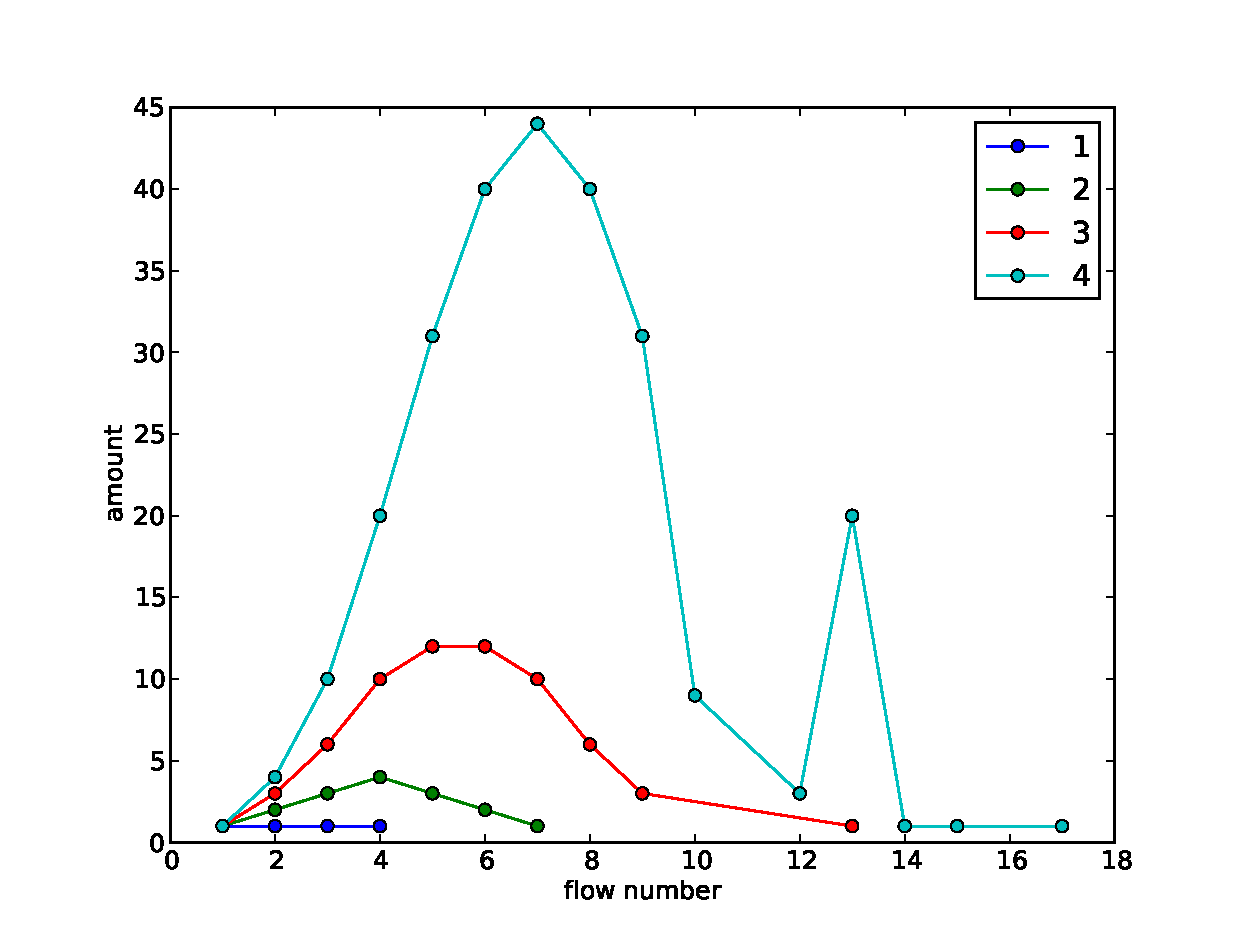
\includegraphics[height=0.9\textheight]{random}
    \end{center}
    \caption{Behaviour with random barcodes.}
    \label{}
  \end{figure}
\end{frame}

\begin{frame}
  \frametitle{Result}

  \begin{table}[]
    \begin{center}
      \begin{tabular}{ll}
        \bt{TTTTT} & \bt{AAAAA}\\
        \bt{CCCCC} & \bt{GGGGG}\\
        \bt{ATTTT} & \bt{CAAAA}\\
        \bt{GCCCC} & \bt{ATGGG}\\
        \bt{CATTT} & \bt{ATGCC}\\
        \bt{ATGCT} & \bt{CATGG}\\
        \bt{GCAAA} & \bt{GCAGG}\\
      \end{tabular}
    \end{center}
    \caption{$14$ flows.}
    \label{}
  \end{table}
\end{frame}

\begin{frame}
  \frametitle{Title of this frame.}

  \begin{figure}[]
    \begin{center}
      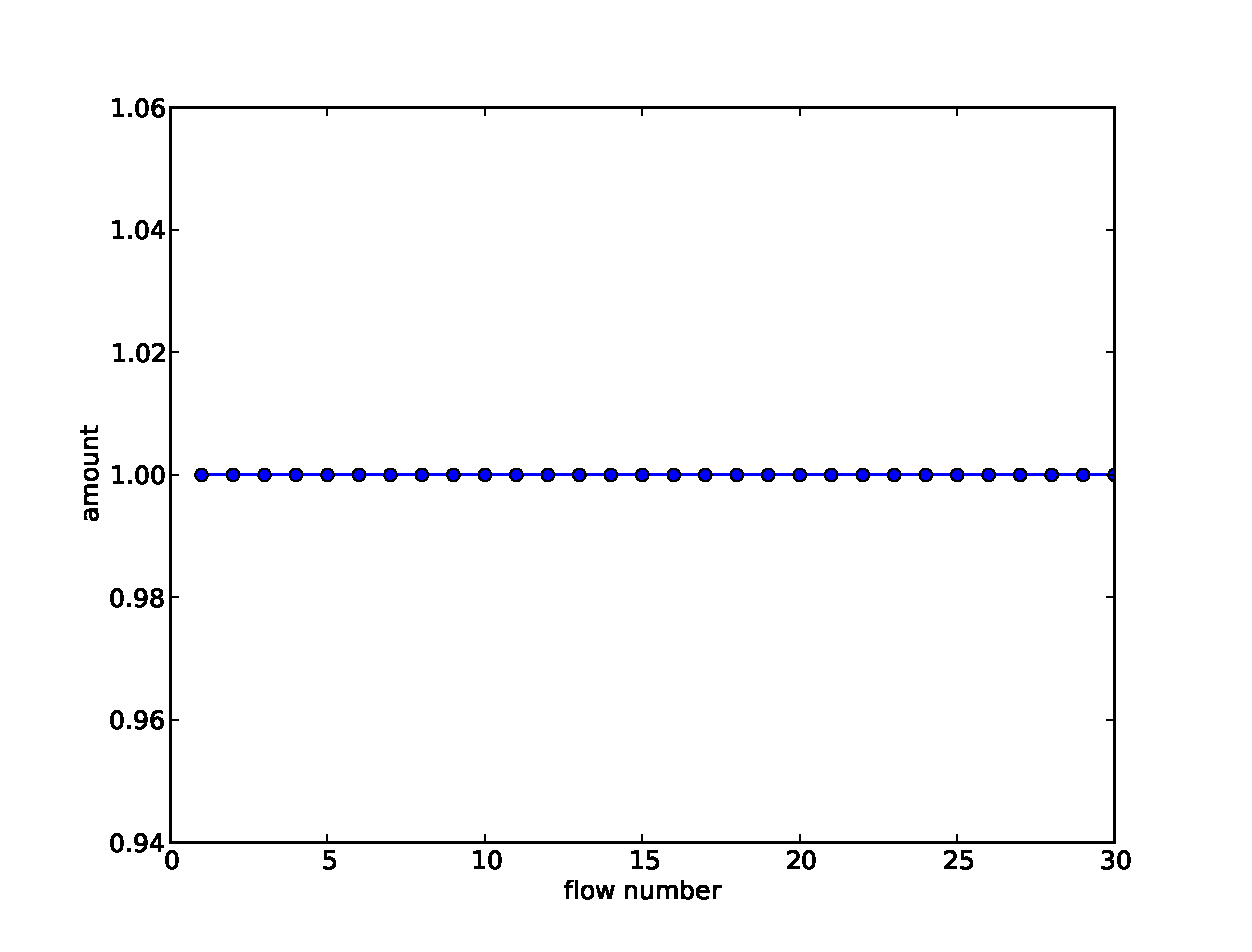
\includegraphics[height=0.9\textheight]{optimised}
    \end{center}
    \caption{Behaviour with optimised barcodes.}
    \label{}
  \end{figure}
\end{frame}

\begin{fframe}
  \frametitle{Title of this frame.}

  \vfill
\end{fframe}

\section{Topic2}
\begin{frame}
  \begin{itemize}
    \item Item 1.
    \item Item 2.
    \pause
    \item Item 3.
    \pause
    \begin{itemize}
      \item Subitem 1.
    \end{itemize}
  \end{itemize}
\end{frame}

\begin{frame}
  The second slide in the same section.
\end{frame}

\begin{frame}[fragile]
  And an example of displaying code, mind the [fragile] option.

  \begin{lstlisting}[caption = {Example input}]
    print "Hello"
  \end{lstlisting}
\end{frame}

\section{Questions?}
\lastpagetemplate
\begin{frame}
  \begin{center}
    Acknowledgements:
    \bigskip
    \bigskip

  \end{center}
\end{frame}

\end{document}
